\documentclass{article}

\usepackage[utf8]{inputenc}
\usepackage[spanish]{babel}

\usepackage{caratula}

\usepackage{subcaption}
\usepackage{graphicx}
\usepackage{dirtytalk}
\usepackage{enumerate}

\usepackage{amssymb}
\usepackage{mathtools}
\usepackage{amsmath}
\usepackage{amsthm}

\usepackage{algorithm}
\usepackage{algpseudocode}
\usepackage{listingsutf8}

\usepackage{float}
\floatplacement{figure}{h!}

\usepackage{geometry}
\usepackage{fixltx2e}
\usepackage{wrapfig}
\usepackage{cite}
\usepackage{dsfont}
\usepackage{ulem}

\usepackage[space]{grffile}

\geometry{
 a4paper,
 total={210mm,297mm},
 left=30mm,
 right=30mm,
 top=30mm,
 bottom=30mm,
 }
 
\usepackage{booktabs}
 
% sql stuff
\usepackage{listings}
\usepackage{courier}
\usepackage{pdflscape}

\newcommand\JSONnumbervaluestyle{\color{blue}}
\newcommand\JSONstringvaluestyle{\color{red}}

% switch used as state variable
\newif\ifcolonfoundonthisline

\makeatletter

\lstdefinestyle{json}
{
  showstringspaces    = false,
  keywords            = {false,true},
  alsoletter          = 0123456789.,
  morestring          = [s]{"}{"},
  stringstyle         = \ifcolonfoundonthisline\JSONstringvaluestyle\fi,
  MoreSelectCharTable =%
    \lst@DefSaveDef{`:}\colon@json{\processColon@json},
  basicstyle          = \ttfamily,
  keywordstyle        = \ttfamily\bfseries,
}

% flip the switch if a colon is found in Pmode
\newcommand\processColon@json{%
  \colon@json%
  \ifnum\lst@mode=\lst@Pmode%
    \global\colonfoundonthislinetrue%
  \fi
}

\lst@AddToHook{Output}{%
  \ifcolonfoundonthisline%
    \ifnum\lst@mode=\lst@Pmode%
      \def\lst@thestyle{\JSONnumbervaluestyle}%
    \fi
  \fi
  %override by keyword style if a keyword is detected!
  \lsthk@DetectKeywords% 
}

% reset the switch at the end of line
\lst@AddToHook{EOL}%
  {\global\colonfoundonthislinefalse}

\newtheorem{theorem}{Teorema}[section]
\newtheorem{corollary}{Corolario}[theorem]
\newtheorem{lemma}{Lema}[theorem]
 
\theoremstyle{definition}
\newtheorem{definition}{Definición}[section]
 
\theoremstyle{remark}
\newtheorem*{remark}{Observación}

\usepackage[dvipsnames]{xcolor}
 
\begin{document}
% Estos comandos deben ir antes del \maketitle
\materia{Bases de Datos} % obligatorio

\titulo{RTP2 \\ Grupo 11}
\subtitulo{NoSQL \\ \today}
\grupo{}

\integrante{Julián Bayardo}{850/13}{julian@bayardo.com.ar} % obligatorio
\integrante{Christian Cuneo}{755/13}{chriscuneo93@gmail.com} % obligatorio 
\integrante{Mauro Cherubini}{835/13}{cheru.mf@gmail.com}
\integrante{Martin Baigorria}{575/14}{martinbaigorria@gmail.com}
 
\maketitle

\tableofcontents

\pagebreak

\section{Introducción}

A partir del diseño realizado anteriormente, el gobierno ahora nos ha solicitado mejorar el tiempo de ejecución de algunas consultas con el objetivo de que los oficiales de policía puedan identificar personas sospechosas rápidamente (sí, cuando se trata de combatir el delito los nanosegundos son importantes). Para ello, nuestro equipo ha decidido utilizar una base de datos no relacional, basada en documentos. Partimos del modelo conceptual desarrollado en el trabajo anterior. Para realizar el nuevo Diagrama de Interrelación de Documentos (DID) necesario para el diseño de nuestra nueva base de datos, tuvimos en cuenta las siguientes consultas que el gobierno desea realizar frecuentemente:

\begin{enumerate}
    \item Cual es el numero promedio de crímenes cometidos por personas que ya han sido encontradas culpables de algún crimen?
    \item Cuales son las personas que se han visto involucradas como testigos en el mayor numero de casos?
    \item Cuales son los casos en los que se han visto involucradas (en cualquier rol) el mayor numero de personas?
    \item Que cantidad, de cada tipo de crimen, ocurrieron en los últimos 45 días?
    \item Cual es el mayor numero de crímenes cometido por alguna persona?
    \item Cuales son las 10 ciudades con mayor numero de crímenes?
    \item Cuales son los casos con mayor numero de evidencias?
\end{enumerate}

La implementación sera realizada en MongoDB.

\subsection{Supuestos}

\begin{itemize}

\item La cantidad de casos que hay en una misma fecha es manejable, lo mismo ocurre para los casos que ocurren en una misma localidad.

\item Cada categoría tiene un nombre de categoría distinto, es decir no hay dos categorías con diferente ID pero que compartan el mismo nombre.

\item Cada rol tiene un nombre de rol distinto, es decir no hay dos roles con diferente ID pero que compartan el mismo nombre.

\item La cantidad de roles y categorías es bastante acotada, de manera que son cantidades bastante manejables.

\item A la hora de realizar aquellas consultas de las cuales se requieran los datos de ciertas personas, no es de interés devolver los datos propios de un oficial (para aquellos que lo sean), a lo sumo interesará saber si es o no es un oficial.

\item El número de casos en los cuales una persona fue culpable, no es excesivamente grande. 

\end{itemize}

\subsection{Diagrama de Entidad Relación (DER)}

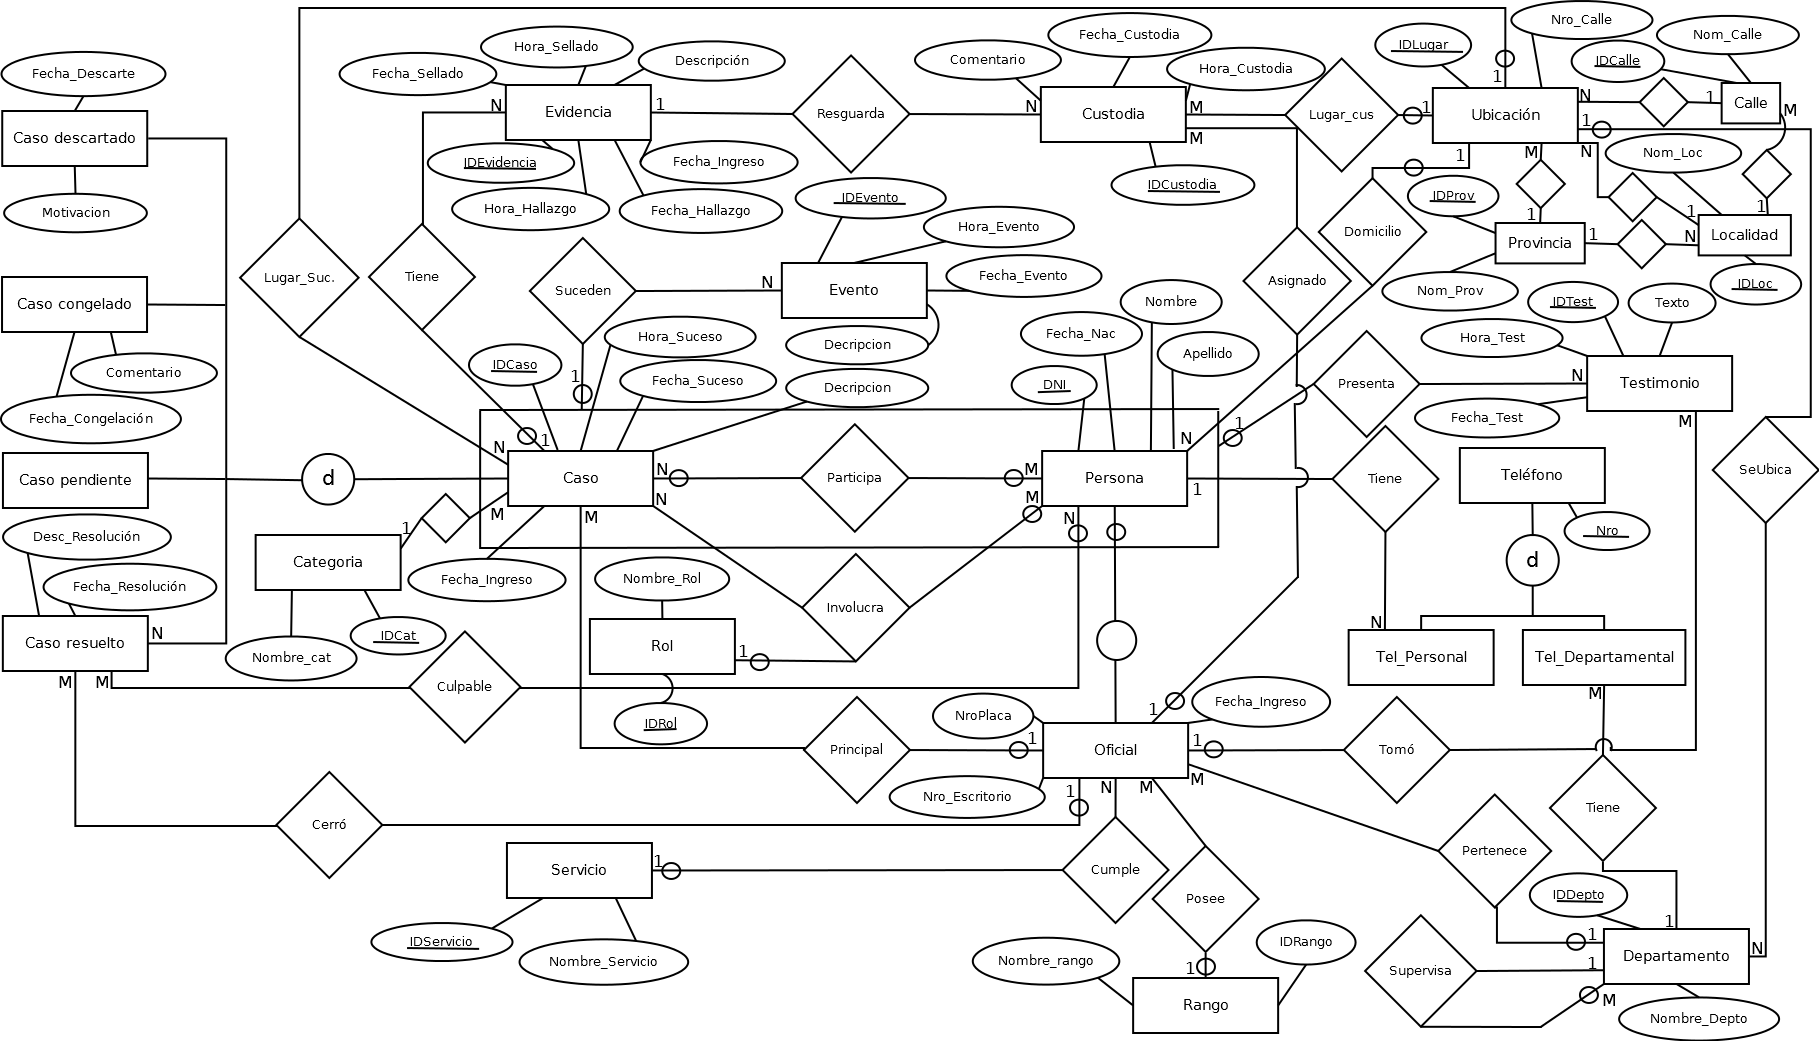
\includegraphics[width=\textheight,height=\textwidth*11/10,angle=90]{der.png}

\subsection{Motivación del diseño}

\begin{itemize}

\item \textbf{Caso:} Este documento esta inspirado en la entidad Caso del DER, pero con algunos agregados que si bien podrían llegar a generar redundancia sirven para optimizar las consultas solicitadas en el enunciado. Para obtener la lista de involucrados en un determinado caso, le agregamos a Caso un arreglo de DNIs que corresponden a aquellas personas que se vieron involucradas bajo cualquier rol con dicho caso, de esta forma no hace falta recorrer la tabla Involucra que teníamos a partir del DER, para saber la identidad cada involucrado. Para poder resolver cuanta evidencia hay por cada caso basta localizar el caso del cual queremos su evidencia, pues esta está embebida en el mismo por medio de un arreglo de documentos que almacena la información pertinente a cada evidencia con la que se relaciona dicho caso. Vale aclarar que si bien se podría haber modelado como anteriormente con las personas (dando un arreglo de IDs) ya que el enunciado solo nos pide saber solo la cantidad de evidencia por cada caso, debido a la intima relación de cada evidencia con su caso nos pareció mas sensato resguardarla toda allí mismo. Análogamente ocurre lo mismo con Categoría y Ubicación, ambas fueron embebidas en Caso, si bien habrá muchos casos que tengan la misma categoría o puedan llegar a coincidir en la ubicación, la redundancia se justifica en que estos son datos básicos de cada caso de manera que es normal pensar que se necesitará acceder a los mismo de manera inmediata.

\item \textbf{Persona:} Este documento esta inspirado en la entidad Persona del DER, a la cual agregamos contenido extra con el fin de optimizar algunas consultas. Para saber lo mas rápido posible cual es el número de crímenes cometidos por persona (que ya hayan cometido algún crimen) y cuales son las personas que han sido testigos en el mayor número de casos, añadimos dos arreglos \textit{Culpable} e \textit{Involucrado}. El arreglo \textit{Culpable} contiene los IDs de todos los casos en los que la persona en cuestión haya sido encontrada culpable; mientras que \textit{Involucrado} contiene para cada entrada un documento que guarda un nombre de rol y un arreglo de IDs correspondientes a los casos en los que la persona en cuestión haya estado involucrado con el rol al cual acompaña. Por ultimo nos pareció sensato embeber la ubicación y teléfono pues son datos básicos que posiblemente se quisieran acceder dado que ya se accedió al documento de una persona.

\item \textbf{Casos\_Por\_Localidad:} La idea detrás de este documento es poder identificar rápido cuales y que cantidad de casos ocurrieron en una localidad especifica. Para ello embebemos la Localidad, teniendo así el nombre de la localidad y su ID, que a su vez será el ID de este nuevo documento. Almacenamos en él además, un arreglo con los IDs de todos los casos cuya ubicación corresponda a la localidad que posee el mismo ID que este documento; de esta manera podemos satisfacer mucho mas rápido aquellas consultas para las cuales necesitamos saber cuantos casos hay por cada localidad.

\item \textbf{Casos\_Por\_Fecha:} Al igual que con la localidad, también se necesita obtener rápidamente los casos que ocurrieron en cierto rango de fechas. Para ello es que este documento adopta como primary key la fecha, y guarda un arreglo de documentos, cuyas entradas contienen el nombre de una categoría y un arreglo con los IDs de todos los casos correspondientes a la misma, que vale aclarar, ocurrieron en la fecha indicada por la primary key. De esta forma para saber cuantos crímenes ocurrieron entre ciertas fechas, alcanza con localizar por fecha aquellos \textit{Casos\_Por\_Fecha} que correspondan y contar la cantidad de IDs de casos contenidos (incluso con la posibilidad de discriminar en la cuenta por categoría).

\end{itemize}

\subsection{Diagrama de Interrelación de Documentos (DID)}

El siguiente DID es un intento por ilustrar gráficamente la inspiración detrás de cada documento JSON modelado para este trabajo práctico. Vale aclarar que si bien para esto nos basamos en el apunte de DID y en las presentaciones vistas en clase, debido a la falta de ejemplos mas complejos es posible que este diagrama no respete o siga alguna convención con la cual no estamos completamente familiarizados. 
%Por esto es que mas adelante en este informe desarrollamos un poco la idea detrás de cada modelo y decisión que consideramos pertinente.

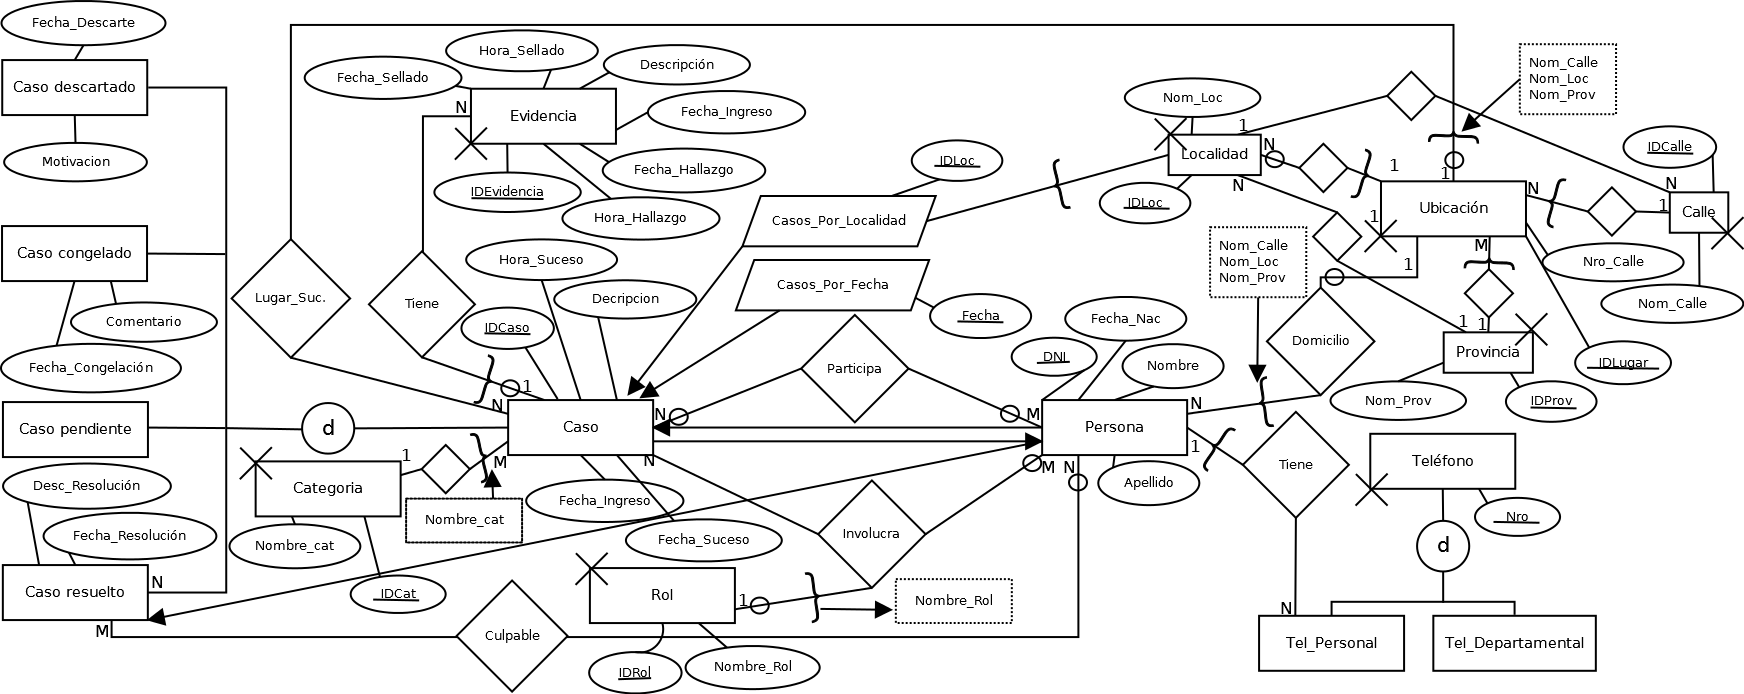
\includegraphics[width=\textheight,height=\textwidth*9/10,angle=90]{DID.png}

\section{Conclusiones}

En este segundo trabajo práctico, en base al modelo conceptual anteriormente desarollado y a los nuevos requerimentos del cliente, pasamos a una base de datos NoSQL orientada a documentos. La idea detrás de este trabajo fue la de poder optimizar determinadas consultas que por diversas razones necesitamos potencialmente acelerar en relación al tiempo de consulta requerido en un modelo relacional, evitando los JOINs. Pudimos notar durante el desarrollo de este trabajo que para poder realizar dicha tarea debíamos modelar los documentos de manera inteligente, para lo que debíamos desestimar la importancia de la redundancia y espacio en disco, que adquirían otra importancia en el trabajo anterior.

Ciertas consultas como las de "todos los documentos que son un máximo global según algún criterio", son más complicadas de expresar en este paradigma: nos requieren utilizar colecciones intermedias para poder guardar los resultados del mapReduce. Si bien esto es algo que implícitamente estaría sucediendo en el paradigma relacional cuando utilizamos una subquery (que hubiera sido la forma de resolver el problema), la sintaxis de la expresión y la carga (en términos de complejidad expuesta al usuario) de la misma resultan ampliamente mayores en MongoDB: nos vemos forzados a crear una colección intermedia, y borrarla luego. A cambio de esta inconveniencia, ganamos en escalabilidad: las consultas mapReduce que escribimos son masivamente paralelizables de una forma casi gratuita en términos de sintaxis, que no es lo que ocurre con SQL.

En conclusión, vimos que MongoDB simplifica ampliamente el proceso de escritura de sistemas escalables: pudimos armar una base de datos optimizada para el caso de uso particular de una forma muy simple, y escribir consultas sobre la misma de una forma más simple aun. Lo interesante es que el esfuerzo de manejar los mecanismos de control de concurrencia y todos sus problemas asociados (así como la transferencia de información entre servidores, etcétera) fue completamente eliminado, permitiéndonos adoptar estrategias de computo embarrassingly parallel de una forma muy sencilla. Además, la flexibilidad del modelo map reduce nos permite expresar cómputos muy complejos de formas comparativamente simples contrastando con la alternativa de utilizar SQL.

\pagebreak

\section{JSON Schemas}

\subsection{Persona}

\lstinputlisting[style=json]{../persona.json}

\pagebreak

\subsection{Caso}

\lstinputlisting[style=json]{../caso.json}

\pagebreak

\subsection{Casos por localidad}

\lstinputlisting[style=json]{../casos_por_localidad.json}

\subsection{Casos por fecha}

\lstinputlisting[style=json]{../casos_por_fecha.json}

\pagebreak

\section{Map Reduce}

\lstinputlisting[style=json]{../functions.js}

\end{document}